\documentclass[11pt,a4paper]{article}
\usepackage[margin=2.5cm]{geometry}
\usepackage{amsmath,amssymb}
\usepackage{booktabs}
\usepackage{enumitem}
\usepackage{xcolor}
\usepackage{tikz}
\usetikzlibrary{positioning,arrows.meta,fit,backgrounds}
\usepackage[colorlinks=true,linkcolor=blue!50!black]{hyperref}

\definecolor{boxbg}{HTML}{EEF3F8}
\definecolor{storeF}{HTML}{CFE3F7}
\definecolor{ctrlF}{HTML}{D7F0D8}
\definecolor{taskF}{HTML}{F6E7C1}
\definecolor{estF}{HTML}{F7D6D6}
\definecolor{ink}{HTML}{43505C}
\definecolor{muted}{HTML}{5A6673}
\newcommand{\idea}[1]{\par\smallskip\noindent\colorbox{boxbg}{\parbox{\dimexpr\linewidth-2\fboxsep}{\textbf{Key idea.} #1}}\par\smallskip}

\title{Planning guide\\[2pt]\large Adding attention (Transformer) components to the learned controllers}
\author{Companion to \texttt{Chapters/4.Implementation.tex} (\texttt{sec:method:model})}
\date{}

\begin{document}
\maketitle

\noindent This is a plan for future work, not part of the thesis model. It
describes how the three learned controllers could use attention, the core
operation of a Transformer, in place of parts of the current graph network,
without changing the problem formulation. Nothing here has been decided or
implemented. It assumes the model as of tags \texttt{[A14]} (learned
messages) and \texttt{[A17]} (per-edge policy head).

\tableofcontents

%----------------------------------------------------------------
\section{Why this is possible without redesigning the model}

After \texttt{[A17]} the model has three separate parts, each with its own
job and its own equation.

\begin{center}
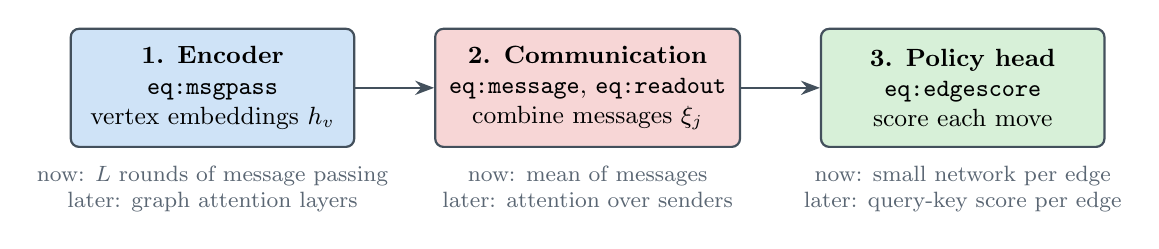
\begin{tikzpicture}[
    box/.style={draw=ink, line width=0.8pt, rounded corners=3pt, align=center,
                font=\small, inner sep=5pt, minimum width=3.6cm, minimum height=1.5cm},
    flow/.style={-{Stealth[length=2.4mm]}, line width=0.9pt, draw=ink},
    note/.style={font=\footnotesize, text=muted, align=center}]
  \node[box, fill=storeF] (enc) {\textbf{1. Encoder}\\ \texttt{eq:msgpass}\\ vertex embeddings $h_v$};
  \node[box, fill=estF, right=1.0cm of enc] (com) {\textbf{2. Communication}\\ \texttt{eq:message}, \texttt{eq:readout}\\ combine messages $\xi_j$};
  \node[box, fill=ctrlF, right=1.0cm of com] (head) {\textbf{3. Policy head}\\ \texttt{eq:edgescore}\\ score each move};
  \draw[flow] (enc) -- (com);
  \draw[flow] (com) -- (head);
  \node[note, below=3pt of enc] {now: $L$ rounds of message passing\\ later: graph attention layers};
  \node[note, below=3pt of com] {now: mean of messages\\ later: attention over senders};
  \node[note, below=3pt of head] {now: small network per edge\\ later: query-key score per edge};
\end{tikzpicture}
\end{center}

\idea{Each part can be replaced by an attention version on its own, and
none of the three touches the problem formulation. The game $\mathcal{M}$,
the observation functions $O_i$, the action space $\mathcal{U}_i$, the
mask, the reward and the training procedure all stay exactly as they are.}

\noindent The three parts are independent because each reads and writes
the same kind of object. The encoder turns vertex features into vertex
embeddings, communication turns messages into one summary per agent, and
the head turns embeddings into one score per legal move. Any replacement
that keeps those inputs and outputs slots in.

%----------------------------------------------------------------
\section{The one rule that must not be broken}

\idea{Change all three learned controllers together, or not at all.}

RQ2 compares the controllers under the claim that they share one encoder
family, one training procedure and one budget, and differ only in their
window (\texttt{[A5]}, \texttt{[A13]}). If only the decentralised
controller got an attention encoder, a difference in results could come
from the encoder, not from the window, and RQ2 would be confounded. So an
attention encoder is either used by all three learned controllers, or run
as a separate, clearly labelled ablation that is never mixed into the main
comparison.

Two further rules keep the design consistent with decisions already made.

\begin{itemize}[leftmargin=*]
  \item \textbf{The windows stay the same.} Attention must be restricted to
        the vertices and agents a controller is already allowed to see.
        Attention over the whole graph for the decentralised controller
        would silently turn it into a centralised one.
  \item \textbf{Communication stays one round.} Stacking attention layers
        over the agent graph would relay what agents beyond the field of
        view send, the same reason \texttt{[A14]} fixed one round.
\end{itemize}

%----------------------------------------------------------------
\section{Swap point 3, the policy head (cheapest, do first)}

\paragraph{Now.} $\mathrm{logit}(\mathrm{move\ to\ } w) = \mathrm{SCORE}_\theta(z_i \Vert h_w \Vert \bar\xi_w)$,
a small fully connected network applied to every outgoing edge.

\paragraph{Attention version.} Score each move by how well the agent's
context matches the vertex it leads to, a query-key product,
\[
  \mathrm{logit}(\mathrm{move\ to\ } w) =
  C \tanh\Bigl( \frac{(W_Q z_i)^\top \, W_K [h_w \Vert \bar\xi_w]}{\sqrt{d_k}} \Bigr),
\]
with learned matrices $W_Q$, $W_K$, key size $d_k$, and a constant $C$
that bounds the logits. The wait score stays $\mathrm{SCORE}^{\mathrm{wait}}_\theta(z_i)$,
or becomes the same product with a learned ``wait'' key. This is the
selection step of the decoder in Kool, van Hoof and Welling (2019), which
also clips logits with $C\tanh$.

\paragraph{Why first.} It is a few lines of code, it changes no input or
output, and it has almost no extra compute. It mainly tests whether a
multiplicative score works better than a small network, so expect a small
effect either way.

%----------------------------------------------------------------
\section{Swap point 2, communication (moderate)}

\paragraph{Now.} $\mathrm{AGG}\{\xi_j(t)\}$ is the mean of the messages
from the agents in $a_i$'s field of view.

\paragraph{Attention version.} Let agent $a_i$ weigh each sender by how
relevant it is,
\[
  m_i = \sum_{j} \beta_{ij}\, W_V \xi_j(t), \qquad
  \beta_{ij} = \mathrm{softmax}_j\Bigl( \frac{(W_Q z_i)^\top W_K \xi_j(t)}{\sqrt{d_k}} + b_{\,d_G(\ell_i(t),\,\ell_j(t))} \Bigr),
\]
where $j$ ranges over the agents with $(a_i,a_j) \in E^{\mathcal{A}}_t$,
and $b_d$ is a learned bias for each hop distance $d \le d_{\mathrm{obs}}$,
so a sender one hop away can count differently from one two hops away.
$m_i$ replaces the mean in \texttt{eq:readout}. With several heads, each
head can attend to a different kind of neighbour (for example, one to
agents in the way, one to agents heading the same way).

\paragraph{What it buys.} A mean treats every sender alike and dilutes one
important message among several unimportant ones. Attention lets the agent
focus on the agent actually in its way. This is the direction of SePar
(\texttt{zhao2025separ}), which \texttt{3.Background.tex} already
discusses, but kept local and one round.

\paragraph{What to watch.} With only a few senders in range, attention and
a mean may perform the same. Compare them on high agent density, where
messages compete.

%----------------------------------------------------------------
\section{Swap point 1, the encoder (largest change)}

\paragraph{Now.} $L$ rounds of message passing over the controller's
window, each vertex combining its neighbours as an unordered set
(\texttt{eq:msgpass}).

\paragraph{Attention version.} Replace each round by a graph attention
layer, where every vertex attends to the other vertices of the same window,
\[
  h_v' = h_v + \sum_{w} \alpha_{vw}\, W_V h_w, \qquad
  \alpha_{vw} = \mathrm{softmax}_w\Bigl( \frac{(W_Q h_v)^\top W_K h_w}{\sqrt{d_k}} + b_{\,d_G(v,w)} \Bigr),
\]
followed by a small feed-forward network and layer normalisation, as in a
standard Transformer layer. $w$ ranges over the window only, the
field of view for the decentralised controller, $Y_q \cup H_q$ for the
section-based one, and the whole graph for the centralised one.

\paragraph{The graph has to be put back in.} Plain attention ignores the
edges, so every vertex looks equally close to every other. The bias
$b_{\,d_G(v,w)}$, one learned number per hop distance, is how the graph
structure re-enters, and it is the standard fix in graph transformers
(Graphormer, Ying et al.\ 2021, uses this kind of distance bias). Two
choices matter here.
\begin{itemize}[leftmargin=*]
  \item Use \emph{relative} information such as hop distance, never
        absolute vertex numbers. Absolute positions would not transfer to a
        different warehouse, the same reason vertex numbers are kept out of
        the features (\texttt{[A15]}, \texttt{[A17]}).
  \item Directed edges matter (one-way aisles). Use the directed distance
        $d_G(v,w)$, which is not symmetric, so attention can tell ``I can
        reach $w$'' from ``$w$ can reach me''.
\end{itemize}

\paragraph{Cost.} Attention over $n$ vertices costs about $n^2$ per layer.
For the decentralised field of view $n$ is small and this is cheap. For the
centralised controller $n = |V|$, so a pass over a large warehouse becomes
expensive, and this grows with warehouse size, while message passing grows
only with the number of edges. Options, in order of preference:
\begin{enumerate}[leftmargin=*]
  \item Restrict each vertex's attention to vertices within a few hops
        (sparse attention). The centralised controller still sees the whole
        graph, because information travels further with each layer, as it
        does now.
  \item Keep message passing in the lower layers and add one attention
        layer on top.
\end{enumerate}
Report the runtime $\kappa_T$ either way, since it is already a dependent
variable and attention will raise it.

\paragraph{This also answers an open point.} \texttt{[A8]} notes that
without pooling, the centralised router does not in practice condition on
the global state, because a vertex embedding only reflects vertices within
$L$ hops. Attention over the whole graph, or a single pooled attention
token, would close that gap directly.

%----------------------------------------------------------------
\section{Where it goes in the code}

In \texttt{slap-mapd-coupling}, all three swaps stay inside
\texttt{models/}.
\begin{description}[leftmargin=*]
  \item[Encoder] \texttt{gnn\_encoder.py} defines \texttt{GNNEncoder} with
        \texttt{num\_rounds}. Add a sibling class, for example
        \texttt{AttentionEncoder}, with the same inputs (vertex features,
        adjacency, window) and the same output (one embedding per vertex),
        plus a config field choosing between them. Precompute the hop
        distances of the window once per step for the bias, the
        all-pairs distances already exist in the simulator.
  \item[Communication] where the readout aggregates messages, replace the
        mean by the attention sum above, behind the same config switch.
  \item[Head] where \texttt{SCORE}$_\theta$ is applied per edge, swap the
        small network for the query-key product.
  \item[Unchanged] \texttt{rl\_module.py} and the masking module only see
        the encoder output and the logits, so they need no change. The
        action space, the mask, the reward and the training loop stay as
        they are.
\end{description}

%----------------------------------------------------------------
\section{How to test it}

\begin{enumerate}[leftmargin=*]
  \item Do the head first, then communication, then the encoder, one at a
        time, so each effect can be measured on its own.
  \item Run each swap as an ablation with the same training budget as the
        baseline, and the same seeds, as \texttt{sec:method:training}
        already requires for the main arms.
  \item Start with the decentralised controller only, as a quick check.
        Before any result enters the RQ2 comparison, apply the same swap to
        all three learned controllers (the rule in Section 2).
  \item Record training time and inference time as well as the outcome
        measures. Attention tends to need more samples and more tuning
        (learning rate, warm-up) than message passing, so a worse result
        after the same budget may mean ``needs more training'', not ``does
        not help''.
\end{enumerate}

%----------------------------------------------------------------
\section{What would change in the thesis}

Only the Method chapter, since the formulation is untouched.
\begin{itemize}[leftmargin=*]
  \item \texttt{sec:method:model}, the equations of whichever part is
        swapped (\texttt{eq:msgpass}, \texttt{eq:readout}, \texttt{eq:edgescore}),
        and \texttt{tab:modelparams} (number of heads, key size, distance
        bias).
  \item \texttt{2.Notation.tex}, new symbols ($W_Q$, $W_K$, $W_V$, $d_k$,
        $b_d$, $\alpha$, $\beta$). Check the letters first, as
        \texttt{AGENTS.md} requires. $\alpha$ is already the storage weight
        on $D$, so the attention weights need other letters.
  \item \texttt{3.Background.tex}, where SePar is discussed, would then be
        cited as a precedent rather than only as a contrast.
  \item \texttt{references.bib}, for Kool et al.\ (2019), and a graph
        transformer paper such as Graphormer, once their details have been
        checked against the papers themselves.
  \item A new \texttt{[Axx]} entry in \texttt{GAPS.md}.
\end{itemize}

%----------------------------------------------------------------
\section{Summary in five lines}

\begin{enumerate}[leftmargin=*]
  \item The encoder, communication and policy head can each become attention on their own.
  \item The problem formulation, action space, mask, reward and training stay unchanged.
  \item Change all three learned controllers together, and keep every window and the single communication round.
  \item Put the graph back into attention with a learned bias per directed hop distance, never with absolute vertex numbers.
  \item Test head, then communication, then encoder, as ablations with the same budget, and report runtime.
\end{enumerate}

\end{document}
